Al fine di rendere più sicuro il sistema già esistente di certificazione della posizione, è stata introdotta la tecnologia blockchain di Algorand, che consente di rendere più sicure alcune operazioni immagazzinando i dati di posizione in blockchain rendendoli così immutabili.

\section{Introduzione}
Il nuovo progetto ha mantenuto parte dell'architettura di base con l'aggiunta di uno smart contract per aumentare i livelli di sicurezza. La sua gestione è controllata da Intecs SpA e sono state elaborate scelte implementative per impedire che lo smart contract non sia in nessun modo modificato o eliminato da terzi\footnote{Lo smart contract è memorizzato in blockchain e non sarà mai realmente eliminato dalla struttura dati. La procedura di eliminazione imposta la variabile booleana "Deleted" associata ai dettagli dello smart contract a True e questo rende impossibile richiamare i metodi dello smart contract.}. La necessità è stata quindi quella di creare un account Algorand ad uso esclusivo dell'azienda, la quale si occuperà anche della gestione di un altro account dello stesso tipo per il sistema centrale. Quest'ultimo componente (il sistema centrale) è unico ed ha il compito di chiamare due metodi dello smart contract: compare\_hash e validate\_snapshot. Infine, sarà necessario anche creare un account Algorand per ogni sistema mobile per poter richiamare il metodo insert\_local\_hash. 

\subsection{Il problema della certificazione degli snapshot}
Durante lo studio della tecnologia Algorand sono state evidenziate alcune incongruenze su quello che doveva essere uno degli obiettivi principali. Si è accennato nell'introduzione che lo scopo del tirocinio fosse quello di certificare la posizione direttamente su blockchain. Questa soluzione non risulta possibile, visto che, per certificare due snapshot è necessario applicare l'algoritmo di allineamento visto nel capitolo precedente e l'implementazione di quest'ultimo nello smart contract risulterebbe troppo complicato e costoso a livello computazionale. Per questa ragione il confronto viene eseguito direttamente dal sistema centrale.

\subsection{Antenna: una componente per simulare la ricezione degli snapshot}
L'antenna è una componente che simula il dispositivo di localizzazione del segnale satellitare (chiamato anche ricevitore) connesso al sistema mobile e alla stazione di riferimento. Nel sistema di base, il sistema mobile e la stazione di riferimento catturano lo snapshot attraverso i satelliti Galileo e calcolano la propria posizione sfruttando queste informazioni (maggiori spiegazioni sono date nel capitolo \ref{3.progetto iniziale}). Il sistema mobile e la stazione di riferimento sono dotati di un orologio atomico perfettamente sincronizzato che permette l'acquisizione dei segnali satellitari nel solito istante. A cadenza di 120 secondi acquisiscono i segnali dai satelliti e nell'istante in cui iniziano a farlo, registrano un timestamp\footnote{Un timestamp è una sequenza di caratteri che rappresentano una data e/o un orario per accertare l’effettivo avvenimento di un certo evento.} che sarà lo stesso per entrambe le macchine. Il timestamp ci risulta utile visto che, a partire dal timestamp associato allo snapshot del sistema mobile è possibile individuare lo snapshot catturato dalla stazione di riferimento e confrontare le due sequenze. Nel nuovo sistema sviluppato che introduce la blockchain, non è possibile che i sistemi mobili e le stazione di riferimento abbiano un orologio atomico sincronizzato visto che si tratta di un prototipo che simula il funzionamento del sistema di certificazione della posizione che non si collega realmente ai satelliti Galileo. Per trovare una soluzione a questo problema, è stata implementata la componente antenna che a cadenza regolare di 120 secondi acquisisce un timestamp e uno snapshot (sequenza di lettere e numeri generato casualmente) e lo invia al sistema mobile e alla stazione di riferimento. Queste due componenti dopo aver ricevuto il timestamp e lo snapshot, sono in grado di simulare lo snapshot da inviare poi al sistema centrale [vedi figura \ref{fig: ricevi_snapshot }]. Genereranno entrambe due file: 
\begin{itemize}
    \item un file zip che al proprio interno avrà il file binario snapshot.bin che contiene lo snapshot in formato binario, ricevuto da antenna.
    \item un file json che conterrà metadati, la cui forma è descritta più avanti.
\end{itemize}

\begin{figure}[h]
\centering
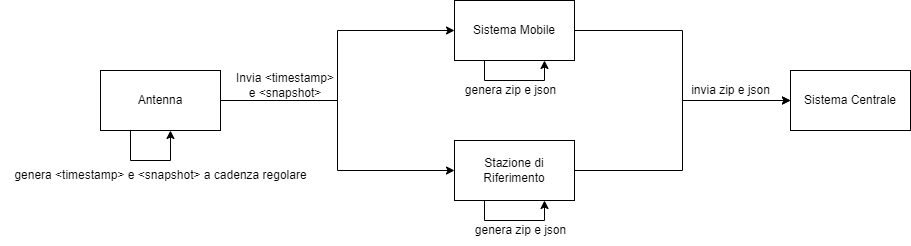
\includegraphics[scale=0.5]{images/ricezione_snapshot.png}
\caption{Un esempio di funzionamento della componente antenna per la ricezione degli snapshot}
\label{fig: ricevi_snapshot }
\end{figure}

\section{Sviluppo dello smart contract}
Gli smart contract in generale sono programmi che vengono archiviati sulla blockchain ed eseguiti quando vengono soddisfatte determinate condizioni; possono generare transazioni di pagamenti, asset e memorizzare valori sulla blockchain e l’archiviazione su questi contratti può essere globale\footnote{L’archiviazione globale è formata dai dati che vengono specificatamente memorizzati sulla blockchain a livello globale.} o locale\footnote{Le variabili locali vengono archiviate nell'account che ha aderito allo smart contract con la fase di opt-in.}. Nella fase di creazione dello smart contract è necessario specificare il numero massimo di variabili locali e globali poiché questi valori non potranno più essere modificati. Lo smart contract implementato è stato allocato con una variabile locale \textit{hash\_snapshot\_sm} e una globale chiamata \textit{Address Sistema Centrale}, entrambe di tipo byteslice (stringa di byte). La variabile globale contiene l'indirizzo pubblico dell'account Algorand del sistema centrale e viene fornita la possibilità di poterla modificare sfruttando il metodo dello smart contract \textit{set\_sistema\_centrale}. Questa variabile globale assicura che i metodi dello smart contract del sistema centrale possano essere effettivamente eseguiti solo dall'account Algorand di quest'ultimo. Infatti, i metodi (\textit{compare\_hash} e \textit{validate\_snapshot}), una volta chiamati, controllano che l'indirizzo del mittente della transazione sia uguale al valore della variabile globale \textit{Address Sistema Centrale}. Questo controllo, certifica che la chiamata di questi due metodi sia un'esclusiva del sistema centrale evitando che chiunque possa richiamarli senza permesso. La variabile locale invece è associata all'account che fa opt-in con lo smart contract creato. Di conseguenza, nel nostro caso, facendo opt-in viene allocato uno spazio di memoria sull'account Algorand per la memorizzazione della variabile locale. Al primo avvio del sistema centrale si effettua una transazione di tipo opt-in per verificare che l'account Algorand di quest'ultimo sia collegato allo smart contract. Per chiarire l'argomento, mostriamo i metodi dello smart contract che abbiamo implementato:
\begin{itemize}
    \item set\_sistema\_centrale: metodo utile nel caso ci sia bisogno di revocare i diritti ad un sistema centrale a favore di un altro. Può essere chiamato solo dall’Account Intecs.
    \item insert\_local\_hash: metodo che prende come argomento una stringa che rappresenta l'hash dello snapshot ricevuto da antenna e lo inserisce nella variabile locale hash\_snapshot\_sm associata all'account Algorand del sistema mobile. Può essere chiamato solo dal sistema mobile. L'hash dello snapshot si calcola applicando la funzione hash sha\_256 \cite{gilbert2003security} direttamente allo snapshot cioè alla stringa ricevuta da antenna.
    \item compare\_hash: metodo utilizzato dall’account sistema centrale per confrontare due byteslice. Confronta la variabile locale di Account sistema mobile con il primo argomento passato hash(snapshot\_sm).
    \item validate\_snapshot: metodo chiamato dall’account sistema centrale che inserisce in blockchain lo snapshot validato.
\end{itemize}


\subsection{Variabile locale dello smart contract}
Con l'operazione di opt-in del sistema mobile allo smart contract, l'account aderisce a quest'ultimo e nel suo account viene allocato lo spazio per le variabili locali nel caso queste siano state specificate nella fase di creazione dello smart contract. Nella figura \ref{fig: statolocale}, mostriamo la chiamata \textit{hash\_snapshot\_sm} attraverso il quale viene assegnato il valore alla variabile \textit{insert\_local\_hash}.

\begin{figure}[!h]
\centering
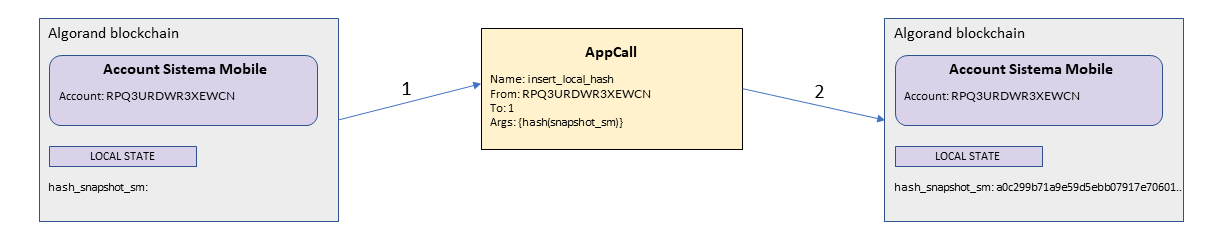
\includegraphics[scale=0.5]{images/local_state.png}
\caption{Un esempio di assegnamento ad una variabile locale}
\label{fig: statolocale}
\end{figure}

\subsection{Gestione degli account Algorand}
Per inviare qualsiasi tipo di transazione, creare smart contract e richiamare i metodi di quest'ultimo è necessario possedere un account Algorand. Poiché nel progetto è stata sfruttata la rete Testnet, gli account vengono creati su questa rete. Il codice per creare un account Algorand sfruttando Python è molto semplice:
\begin{pythoncode}
import json
from algosdk import account, mnemonic

acct = account.generate_account()
address1 = acct[1]
print("Account 1")
print(address1)
mnemonic1 = mnemonic.from_private_key(acct[0])
print("mnemonic1 = \"{}\"".format(mnemonic1))

# l'output del terminale sarà simile a:
# Account 1
# KECA5Z2ZILJOH2ZG7OPKJ5KMFXP5XBAOC7H36TLPJOQI3KB5UIYUD5XTZU
# mnemonic1 = "consider round clerk soldier hurt dynamic floor video
# output spoon deliver virtual zoo inspire rubber doll nose warfare 
# improve abstract recall choice size above actor"
\end{pythoncode}
La creazione dell'account restituisce una chiave pubblica e una privata. La pubblica è visibile a tutti mentre la privata va mantenuta nascosta agli altri utenti di Algorand. Quando si vuole inviare una transazione, la chiave pubblica diventa utile per creare la transazione non firmata. La privata invece si utilizza per firmare la transazione, un passo fondamentale per evitare che chiunque possa effettuare transazioni con account di altri utenti. La blockchain di Algorand supporta anche le chiavi mnemoniche che vengono generate durante la registrazione dell'account. Una chiave mnemonica è un modello di 25 parole che rappresenta al meglio la chiave privata ed esegue le stesse funzioni di quest'ultima. Una volta creato l'account, il suo Wallet deve essere ricaricato con Algos, la moneta della Testnet e l'operazione avviene sfruttando l'Algorand Dispenser. E' sufficiente utilizzare la chiave pubblica dell'account Algorand per poter ricaricare il Wallet associato [vedi figura \ref{fig: dispenseralgorand}].
\begin{figure}[!h]
\centering
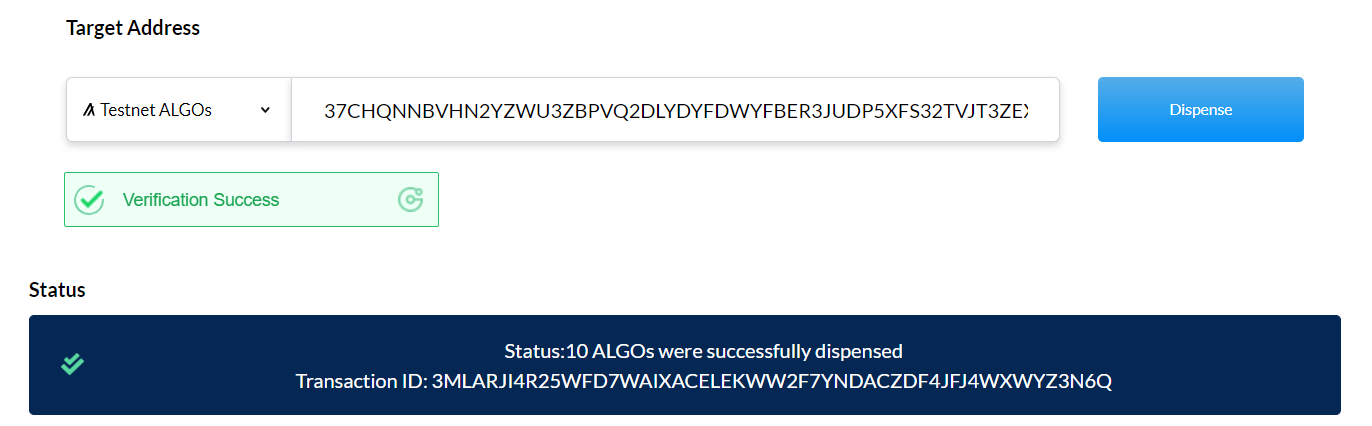
\includegraphics[scale=0.5]{images/algorand_dispenser.png}
\caption{Un esempio di utilizzo del Dispenser di Algorand}
\label{fig: dispenseralgorand}
\end{figure}
Questo tipo di operazione deve essere effettuata per creare l'account Intecs, utilizzato per creare, gestire e poter chiamare il metodo \textit{set\_sistema\_centrale} dello smart contract. Si crea anche l'account associato al sistema centrale che ci servirà per chiamare i metodi \textit{compare\_hash} e \textit{validate\_snapshot}. Infine è necessario un account Algorand per ogni sistema mobile funzionante, per poter richiamare il metodo \textit{insert\_local\_hash} dello smart contract. La stazione di riferimento e l'antenna non interagiscono con la blockchain e lo smart contract creato, non necessitano quindi di un Algorand account.
Di seguito vediamo anche un esempio completo che illustra come inviare rapidamente una semplice transazione:
\begin{pythoncode}
import json
import base64
from algosdk import account, mnemonic, constants
from algosdk.v2client import algod
from algosdk.future import transaction


def generate_algorand_keypair():
    private_key, address = account.generate_account()
    print("My address: {}".format(address))
    print("My private key: {}".format(private_key))
    print("My passphrase: {}".format(mnemonic.from_private_key(private_key)))

# Write down the address, private key, and the passphrase for later usage
generate_algorand_keypair()

def first_transaction_example(private_key, my_address):
    algod_address = "http://localhost:4001"
    algod_token = 64 * "a"
    algod_client = algod.AlgodClient(algod_token, algod_address)

    print("My address: {}".format(my_address))
    account_info = algod_client.account_info(my_address)
    print("Account balance: {} microAlgos".format(account_info.get('amount')))

    # build transaction
    params = algod_client.suggested_params()
    # comment out the next two (2) lines to use suggested fees
    params.flat_fee = constants.MIN_TXN_FEE 
    params.fee = 1000
    receiver = "HZ57J3K46JIJXILONBBZOHX6BKPXEM2VVXNRFSUED6DKFD5ZD24PMJ3MVA"
    amount = 100000
    note = "Hello World".encode()

    unsigned_txn = transaction.PaymentTxn(my_address, params, receiver, amount, 
    None, note)

    # sign transaction
    signed_txn = unsigned_txn.sign(private_key)

    # submit transaction
    txid = algod_client.send_transaction(signed_txn)
    print("Signed transaction with txID: {}".format(txid))

    # wait for confirmation 
    try:
        confirmed_txn = transaction.wait_for_confirmation(algod_client, txid, 4)  
    except Exception as err:
        print(err)
        return

    print("Transaction information: {}".format(
        json.dumps(confirmed_txn, indent=4)))
    print("Decoded note: {}".format(base64.b64decode(
        confirmed_txn["txn"]["txn"]["note"]).decode()))

    print("Starting Account balance: {} microAlgos".format(account_info.get
    ('amount')) )
    print("Amount transfered: {} microAlgos".format(amount) )    
    print("Fee: {} microAlgos".format(params.fee) ) 


    account_info = algod_client.account_info(my_address)
    print("Final Account balance: {} microAlgos".format(account_info.get
    ('amount')) + "\n")

# replace private_key and my_address with your private key and your address.
first_transaction_example(private_key, my_address)
\end{pythoncode}

\subsection{Principio di funzionamento generale}
Vediamo di seguito, attraverso una rappresentazione grafica [vedi figura \ref{fig: architetturasistema }], il funzionamento del nuovo sistema realizzato che introduce la tecnologia blockchain. Nella figura per semplicità, non sono state inserite le frecce di conferma transazione del metodo dello smart contract insert\_local\_hash e di compare\_hash.

\begin{figure}[!h]
\centering
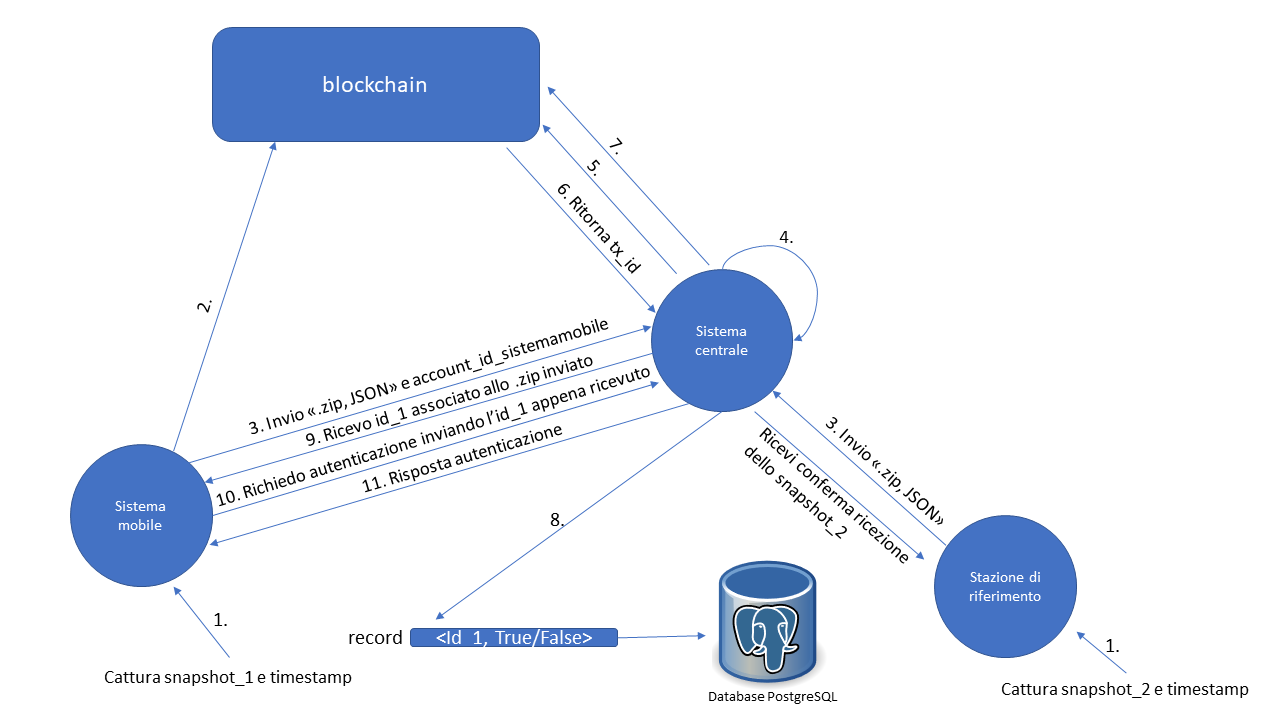
\includegraphics[scale=0.5]{images/schema progetto con blockchain v2.png}
\caption{Architettura del nuovo sistema}
\label{fig: architetturasistema }
\end{figure}

\begin{itemize}
\item 1: la componente antenna invia lo snapshot\_1 al sistema mobile e lo snapshot\_2 alla stazione di riferimento insieme al timestamp (sia lo snapshot che il timestamp sono uguali per entrambi).
\item 2: il sistema mobile invoca il metodo \textit{insert\_local\_hash} dello smart contract passandogli come argomento l'hash dello snapshot\_1 ricevuto da antenna. Il risultato del passo 2 è che l'account Algorand di sistema mobile scrive sulla propria variabile locale hash\_snapshot\_sm il risultato della funzione hash sha\_256 applicata a snapshot\_1.
\item 3: dopo aver acquisito lo snapshot e il timestamp da antenna, il sistema mobile memorizza lo snapshot in un file all'interno di un archivio zip, genera le informazioni di posizione e insieme al timestamp le inserisce in un file JSON per poi inviarle al sistema centrale assieme al proprio indirizzo Algorand (chiave pubblica). Anche la stazione di riferimento, eseguendo le medesime procedure, invierà un file zip e un file JSON.
\item 4: il sistema centrale confronta lo snapshot ricevuto al passo 3 dal sistema mobile e dalla stazione di riferimento.
\item 5: il sistema centrale dopo aver verificato l'uguaglianza degli snapshot al passo 4 può chiamare il metodo dello smart contract \textit{compare\_hash} con i seguenti parametri:
\begin{itemize}
    \item hash(snapshot\_1): lo calcola sfruttando lo snapshot\_1 ottenuto al passo 3.
    \item account\_id\_sistemamobile: lo ottiene al passo 3 e gli serve per accedere alla variabile locale di sistema mobile per acquisire l’hash\_snapshot\_sm e confrontarlo con il primo parametro passato.
\end{itemize}
In pratica lo smart contract valida lo snapshot\_1 controllando che non sia stato alterato al passo 3.
\item 6: se la verifica che lo snapshot\_1 non sia stato alterato al passo 3 è andata a buon fine, viene restituita la transaction\_id (tx\_id) della transazione effettuata al passo 5.
\item 7: non appena il sistema centrale riceve al passo 6 la tx\_id è sicuro che lo snapshot\_1 non sia stato alterato. E' possibile quindi far confrontare lo snapshot\_1 (ricevuto dal sistema mobile) con lo snapshot\_2 (ricevuto dalla stazione di riferimento) al sistema centrale, ed inviare poi, nel caso l'operazione vada a buon fine, una transazione di conferma validazione alla blockchain sfruttando il metodo \textit{validate\_snapshot} dello smart contract che conterrà le seguenti informazioni nel campo nota:
\begin{itemize}
    \item l'id dello snapshot
    \item l'hash dello snapshot del sistema mobile
    \item l'account address del sistema mobile
    \item il timestamp
    \item i dati di posizione dello snapshot certificato (latitudine, longitudine, altitudine)
\end{itemize}
\item 8: al passo 8 viene salvato in un database PostgreSQL interno al sistema centrale il record <id\_1, True/False> dove: l’id\_1 rappresenta l’identificatore univoco del file zip ricevuto da sistema mobile e il secondo campo contiene un booleano che è impostato a True se lo snapshot ricevuto dal sistema mobile non è stato alterato, False altrimenti. Questo meccanismo consente al sistema mobile di poter richiedere l’autenticazione dell’id dello snapshot al sistema centrale quando vuole senza necessità che quest'ultimo ogni volta effettui nuovamente le varie operazioni di confronto tra snapshot.
\item 9: al passo 9 il sistema centrale invia l'id che aveva precedentemente associato allo snapshot (file binario) ricevuto dal sistema mobile a quest'ultimo.
\item 10: il sistema mobile attraverso l'interfaccia a linea di comando cli può richiedere in ogni momento le informazioni di autenticazione dello snapshot tramite l'id ricevuto al passo 8.
\item 11: il sistema centrale invia l’esito dell'autenticazione della posizione al sistema mobile che può essere positivo e in quel caso significa che la posizione è stata autenticata correttamente, altrimenti significa che lo snapshot ricevuto dal sistema mobile è stato corrotto.
\end{itemize}

\subsection{Interazione con la Blockchain}
Il diagramma di sequenza in figura \ref{fig: diagramactivity1} mostra chiaramente le varie interazioni con la blockchain e più nel dettaglio le chiamate che vengono effettuate allo smart contract. Nel progetto di base, il sistema mobile e la stazione di riferimento sono sincronizzati con un orologio atomico che a cadenza regolare di 120 secondi calcola un timestamp \footnote{Un timestamp è una sequenza di caratteri che rappresentano una data e/o un orario per accertare l'effettivo avvenimento di un certo evento.} e inizia a registrare il segnale proveniente dai satelliti Galileo per circa 5 secondi. Questa procedura viene simulata tramite l'invio da parte del sistema antenna di un timestamp e di uno snapshot rispettivamente al sistema mobile e alla stazione di riferimento a cadenza di 120 secondi. Il compito del sistema mobile a questo punto sarà quello di costruire il file zip con all'interno il file snapshot.bin che contiene lo snapshot ricevuto poco fa. 
\begin{figure}[!h]
\centering
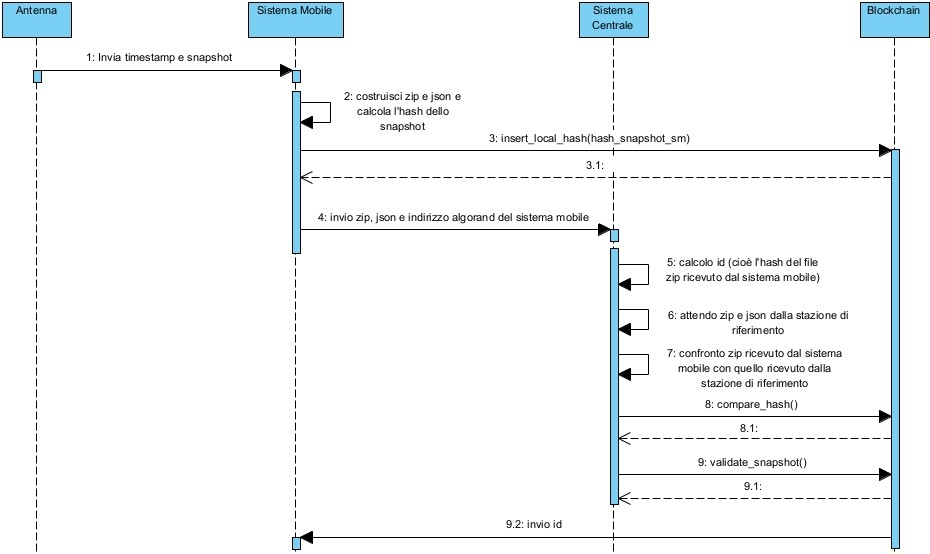
\includegraphics[scale=0.6]{images/Sequence Diagram - scambio msg con blockchain.jpg}
\caption{Diagramma di sequenza dell'interazione con lo smart contract}
\label{fig: diagramactivity1}
\end{figure}\\
Il sistema mobile costruisce anche il file json dei metadati a partire dal timestamp e avrà la seguente forma:\\
\lstinputlisting[label= cod: metadati, caption= esempio di dati di posizione contenuti nel file json dei metadati, language=json, basicstyle=\small]{listing/sourceCode/metadati.json}
Dove i parametri di latitudine, longitudine e altitudine vengono generati casualmente. Lo snapshot reale e cioè quello catturato dai satelliti Galileo, contiene molti altri parametri, ma visto che si tratta di una simulazione solo a scopo di progetto, quelli utilizzati sono sufficienti. Sfruttando la funzione sha\_256 è possibile calcolare l'hash dello snapshot semplicemente applicandola a snapshot.bin che si trova all'interno del file zip generato. E' a questo punto che viene chiamato il metodo dello smart contract \textit{insert\_local\_hash} il cui argomento passato è l'hash dello snapshot appena calcolato. Il sistema mobile invierà i due file zip, json e il proprio indirizzo Algorand al sistema centrale, il quale calcolerà l'id dello snapshot appena ottenuto tramite il calcolo dell'hash del file zip del sistema mobile. Quando il sistema centrale è sicuro di aver ricevuto il file zip e json anche dalla stazione di riferimento può confrontare lo zip del sistema mobile con quello ricevuto dalla stazione di riferimento e chiamare il metodo \textit{compare\_hash} con i seguenti argomenti: hash(snapshot\_1) che lo calcola sfruttando lo snapshot\_1 ottenuto al passo 3 e l'account\_id\_sistemamobile  (anche questo ottenuto al passo 3) che utilizza per accedere alla var. locale di sistema mobile per acquisire l’hash\_snapshot\_sm e confrontarlo con il primo argomento passato. Questa operazione accerta che lo snapshot ottenuto dal sistema mobile non sia stato alterato nell'invio. Se anche questo metodo è andato a buon fine si può certificare lo snapshot di partenza attraverso la chiamata di \textit{validate\_snapshot} e registrare la posizione in blockchain, rendendola di fatto, immutabile.

\section{Sistema Centrale}
Il sistema centrale rappresenta il modulo più importante perché svolge molteplici compiti. Esso infatti, comunica sia con il sistema mobile che con la stazione di riferimento per ottenere i file zip e JSON degli snapshot. Ne effettua anche il salvataggio per poi essere in grado di poterli confrontare ed eventualmente certificare la posizione.
A livello di comunicazione sono stati implementati tre server TCP, ognuno gestito da un diverso thread in continuo ascolto. Elenchiamo di seguito i tre server:
\begin{itemize}
    \item server\_sm: server TCP che comunica con il sistema mobile per la ricezione dei file zip e JSON. Rimane in ascolto di nuove connessioni da parte del sistema mobile e non appena ne arriva una, avvia il thread "thread\_sm" per gestirla.
    \item server\_sr: server TCP che comunica con la stazione di riferimento per la ricezione dei file JSON e zip. Rimane in ascolto di nuove connessioni da  parte dei sistemi mobile e non appena ne arriva una, avvia il thread "thread\_sr" per gestirla.
    \item server\_sm\_cli: server TCP che comunica con il sistema mobile per la ricezione degli id, l'invio dell'esito dell'autenticazione dello snapshot e della lista di tutti gli id ricevuti alla cli. Rimane in ascolto di nuove connessioni da parte dei sistemi mobile. Non appena si avvia un sistema mobile, questo si collegherà in automatico al server. Infatti, il server avvierà un thread "thread\_sm\_cli" che gestirà autonomamente la comunicazione con quel sistema mobile.
\end{itemize}
Ciascuno di questi server quindi, non appena riceve una richiesta dal sistema mobile o dalla stazione di riferimento per aprire una nuova comunicazione, avvierà un thread per la gestione della connessione.

\subsection{File di configurazione}
Nella cartella di sistema\_centrale si trova anche il file info\_algorand.json che contiene i parametri fondamentali per potersi collegare alla blockchain e allo smart contract. 
\lstinputlisting[label= cod: request, caption= esempio del contenuto nel file info\_algorand.json, language=json, basicstyle=\small]{listing/sourceCode/info_algorand.json}

In sintesi, contiene i campi dell'account Algorand del sistema centrale e l'id della dApp creata da Intecs.

\subsection{Persistenza dei dati}
\subsubsection{Database PostgreSQL}
Il sistema centrale memorizza gli id degli snapshot insieme all'esito dell'autenticazione di questi. L'id si ottiene calcolando l'hash del file zip ricevuto dal sistema mobile mentre l'esito dipenderà dal confronto dello snapshot contenuto dal file zip con quello ricevuto dalla stazione di riferimento. Il valore di esito sarà un valore booleano True o False. Il record <id, esito> verrà a questo punto inserito nel database di tipo PostgreSQL e servirà al sistema centrale nel momento in cui il sistema mobile effettuerà una richiesta di autenticazione dello snapshot. Il sistema centrale memorizza poi gli snapshot e i metadati in due database (object storage e database metadati).

\subsubsection{Salvataggio dei file zip e JSON}
Il sistema centrale come sappiamo riceve a intervalli regolari coppie di zip e JSON dai sistemi mobili e dalle stazioni di riferimento e quest'ultimi vengono memorizzati. Per mapparli correttamente vengono mantenuti aggiornati due file all'interno della directory che contiene anche i file zip e JSON. Essi sono:
\begin{itemize}
    \item object\_storage: è un file JSON che contiene le coppie <id,path> dei file zip
    \item metadati.json: è un file JSON che contiene le coppie <id,path> dei file JSON
\end{itemize}

\section{Sistema Mobile}
Il sistema mobile rimane in ascolto degli snapshot da antenna. Come già detto in precedenza, riceve un timestamp e uno snapshot a cadenza regolare e comunica con il sistema centrale tramite connessione TCP per l'invio dei file zip e JSON degli snapshot. Ha un ruolo da intermediario tra la Cli\footnote{La Cli è un programma implementato con un'interfaccia a linea di comando utilizzato per poter richiedere informazioni sugli snapshot e sarà introdotto nel capitolo \ref{5.cli e intecs}.} e il sistema centrale, ma questo lo approfondiremo meglio nel capitolo \ref{capitolo_cli}.

\subsection{File di configurazione}
Nella cartella di sistema\_mobile dove si trova il file sistemamobile.py è presente anche il file di configurazione info\_algorand.json che contiene l'indirizzo dell'account Algorand del sistema mobile e l'id dell'applicazione creata da Intecs SpA. 
\lstinputlisting[label= cod: metadati1, caption= esempio del contenuto nel file info\_algorand.json, language=json, basicstyle=\small]{listing/sourceCode/info_algorand_sm.json}

\subsection{Salvataggio dei dati}
Viene mantenuto un file chiamato id\_list di tipo JSON che su ogni riga contiene alcune informazioni riferite ad un particolare id, ciascuna informazione è delimitata da uno spazio dove la prima informazione rappresenta l'identificatore dello snapshot. Il calcolo dell'identificatore (id) si ottiene applicando la funzione sha\_256 a 'snapshot.bin' all'interno del file zip ricevuto dal sistema mobile. Le due informazioni successive rappresentano rispettivamente la data e l'ora di ricezione dell'identificatore. L'ultimo parametro invece rappresenta un valore booleano che vale True se la certificazione della posizione è avvenuta correttamente e vale False altrimenti [vedi figura \ref{fig: record_id_list }].

\begin{figure}[!h]
\centering
\includegraphics[scale=0.8]{images/record id\_list.png}
\caption{Un esempio di record di id\_list}
\label{fig: record_id_list }
\end{figure}

\section{Stazione di Riferimento}
Come per il sistema mobile anche questa componente rimane in ascolto di timestamp e snapshot dalla componente antenna e comunica con il sistema centrale tramite connessione TCP per l’invio dei file zip e JSON degli snapshot.

\section{Struttura delle cartelle e dei file del progetto}
La cartella \textbf{antenna} contiene i seguenti file:
\begin{itemize}
    \item Dockerfile
    \item config.json
\end{itemize}
La cartella \textbf{intecs} contiene i seguenti file:
\begin{itemize} 
    \item intecs.py 
    \item config.json 
\end{itemize}
La cartella \textbf{sistema\_mobile} contiene i seguenti file e cartelle:
\begin{itemize}
    \item sistemamobile.py 
    \item Dockerfile 
    \item utility.py 
    \item info\_algorand.json
    \item \textbf{cli}
        \begin{itemize}
            \item cli.py
            \item Dockerfile
        \end{itemize}
    \item \textbf{cli v2}
        \begin{itemize}
            \item cli.py 
            \item config.json 
        \end{itemize}
\end{itemize}
La cartella \textbf{sistema\_centrale} contiene i seguenti file:
\begin{itemize}
    \item sistemacentrale.py 
    \item database\_library.py 
    \item Dockerfile 
    \item utility.py 
    \item info\_algorand.json 
\end{itemize}
La cartella \textbf{stazione\_di\_riferimento} contiene i seguenti file:
\begin{itemize}
    \item stazioneriferimento.py 
    \item Dockerfile 
    \item utility.py 
\end{itemize}

\section{Docker}
Il nuovo sistema di certificazione della posizione è stato sviluppato sfruttando Docker Desktop su ambiente Windows. Per far funzionare il progetto con Docker è necessario aver installato sul proprio computer Docker e Docker Compose \cite{dockerinstall}.

\subsection{Avvio del progetto}
E' possibile avviare il progetto di simulazione lanciando il comando \textit{docker-compose up} dalla cartella principale che contiene il file docker-compose.yml.

\subsection{Struttura dei container}
I container di cui si fa uso nel progetto di simulazione sono cinque: 
\begin{itemize}
    \item il sistema centrale
    \item il sistema mobile
    \item la stazione di riferimento
    \item la cli
    \item il database Postgres
\end{itemize}

\subsection{Ordine di avvio}
L'ordine di avvio dei container è il seguente:
\begin{enumerate}
    \item database Postgres
    \item sistema centrale
    \item sistema mobile
    \item cli
    \item stazione di riferimento
\end{enumerate}

\section{Cli - Avvio con Docker Desktop}
Se il progetto è stato eseguito con docker-compose e vogliamo avviare il programma Cli è necessario utilizzare Docker Desktop. Assicurandosi di aver avviato il progetto con il comando \textit{docker-compose up} dalla cartella principale del progetto che contiene il file docker-compose.yml, possiamo procedere all'avvio della Cli. Selezioniamo dalla lista dei container del progetto il container riferito alla Cli e clicchiamo sull'icona del terminale CLI [vedi figura \ref{fig: docker_2 }].
\begin{figure}[!h]
\centering
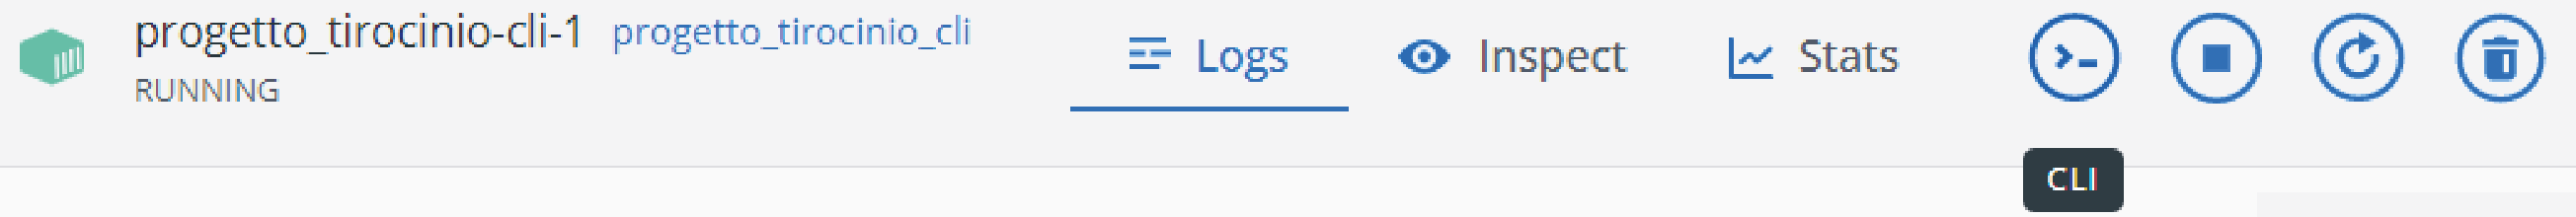
\includegraphics[scale=0.7]{images/docker_2.png}
\caption{Schermata che mostra il pulsante del terminale CLI}
\label{fig: docker_2 }
\end{figure}\\
E' sufficiente, arrivati a questo punto, eseguire dalla console appena aperta il comando \textit{python cli.py} per avviare il programma Cli, come nella figura \ref{fig: docker_3 }.
\begin{figure}[h]
\centering
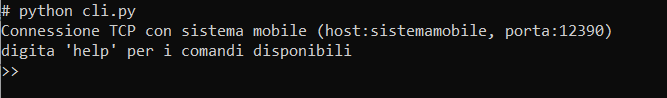
\includegraphics[scale=0.9]{images/docker_3.png}
\caption{Avvio della Cli da Docker Desktop}
\label{fig: docker_3 }
\end{figure}
